%!TEX root = paper.tex

\section{System Architecture}
\label{sec:architecture}

In this section we lay out the architecture of Flink as a software stack, and as a distributed system. While Flink's stack of APIs continues to grow, we can distinguish four main layers: deployment, core, APIs, and libraries.

\para{Flink's Runtime and APIS.} Flink's software stack can be seen in \autoref{fig:stack}. The core of Flink is the distributed dataflow engine, which executes dataflow programs. A Flink runtime program is a DAG of stateful operators connected with data streams. There are two core APIs in Flink: the DataSet API for processing finite data sets (often referred to as “batch processing”), and the DataStream API for processing potentially unbounded data streams (often referred to as “stream processing”). Flink’s core runtime engine can be seen as a streaming dataflow engine, and both the DataSet and DataStream APIs create runtime programs executable by the engine. As such, it serves as the common fabric to abstract both bounded (batch) and unbounded (stream) processing. On top of the core APIs, Flink bundles domain-specific libraries and APIs that generate DataSet and DataStream API programs (currently FlinkML, Gelly, and Table). 

As depicted in \autoref{fig:process-model}, a Flink cluster comprises three types of processes: the client, the JobManager (JM - master), and one or more TaskManagers (TM - workers). The client takes the program code, transforms it to a dataflow graph, and submits that to the JobManager. This transformation phase also examines the data types (schema) of the data exchanged between operators and creates serializers and other type/schema specific code. DataSet programs additionally go through a cost-based query optimization phase, similar to the physical optimizations performed by relational query optimizers (more details in \autoref{sec:batch}).

The JobManager coordinates the distributed execution of the dataflow. It tracks the state and progress of each operator and stream, schedules new operators, and coordinates checkpoints and recovery. In a high-availability setup, the JobManager persists a minimal set of metadata at each checkpoint to a fault-tolerant storage, such that a standby JobManager can reconstruct the checkpoint and recover the dataflow execution from there (see \autoref{sec:fault-tolerance}). The actual data processing takes place in the TaskManagers. A TaskManager executes one or more operators that produce streams, and reports on their status to the JobManager. The TaskManagers maintain the buffer pools to buffer or materialize the streams, and the network connections to exchange the data streams between operators.


\begin{figure}[t!]
\begin{minipage}{1.1\linewidth}
      \centering
      \hspace{-0.1\linewidth}
      \begin{minipage}{0.48\linewidth}
          \begin{figure}[H]
              \centering
			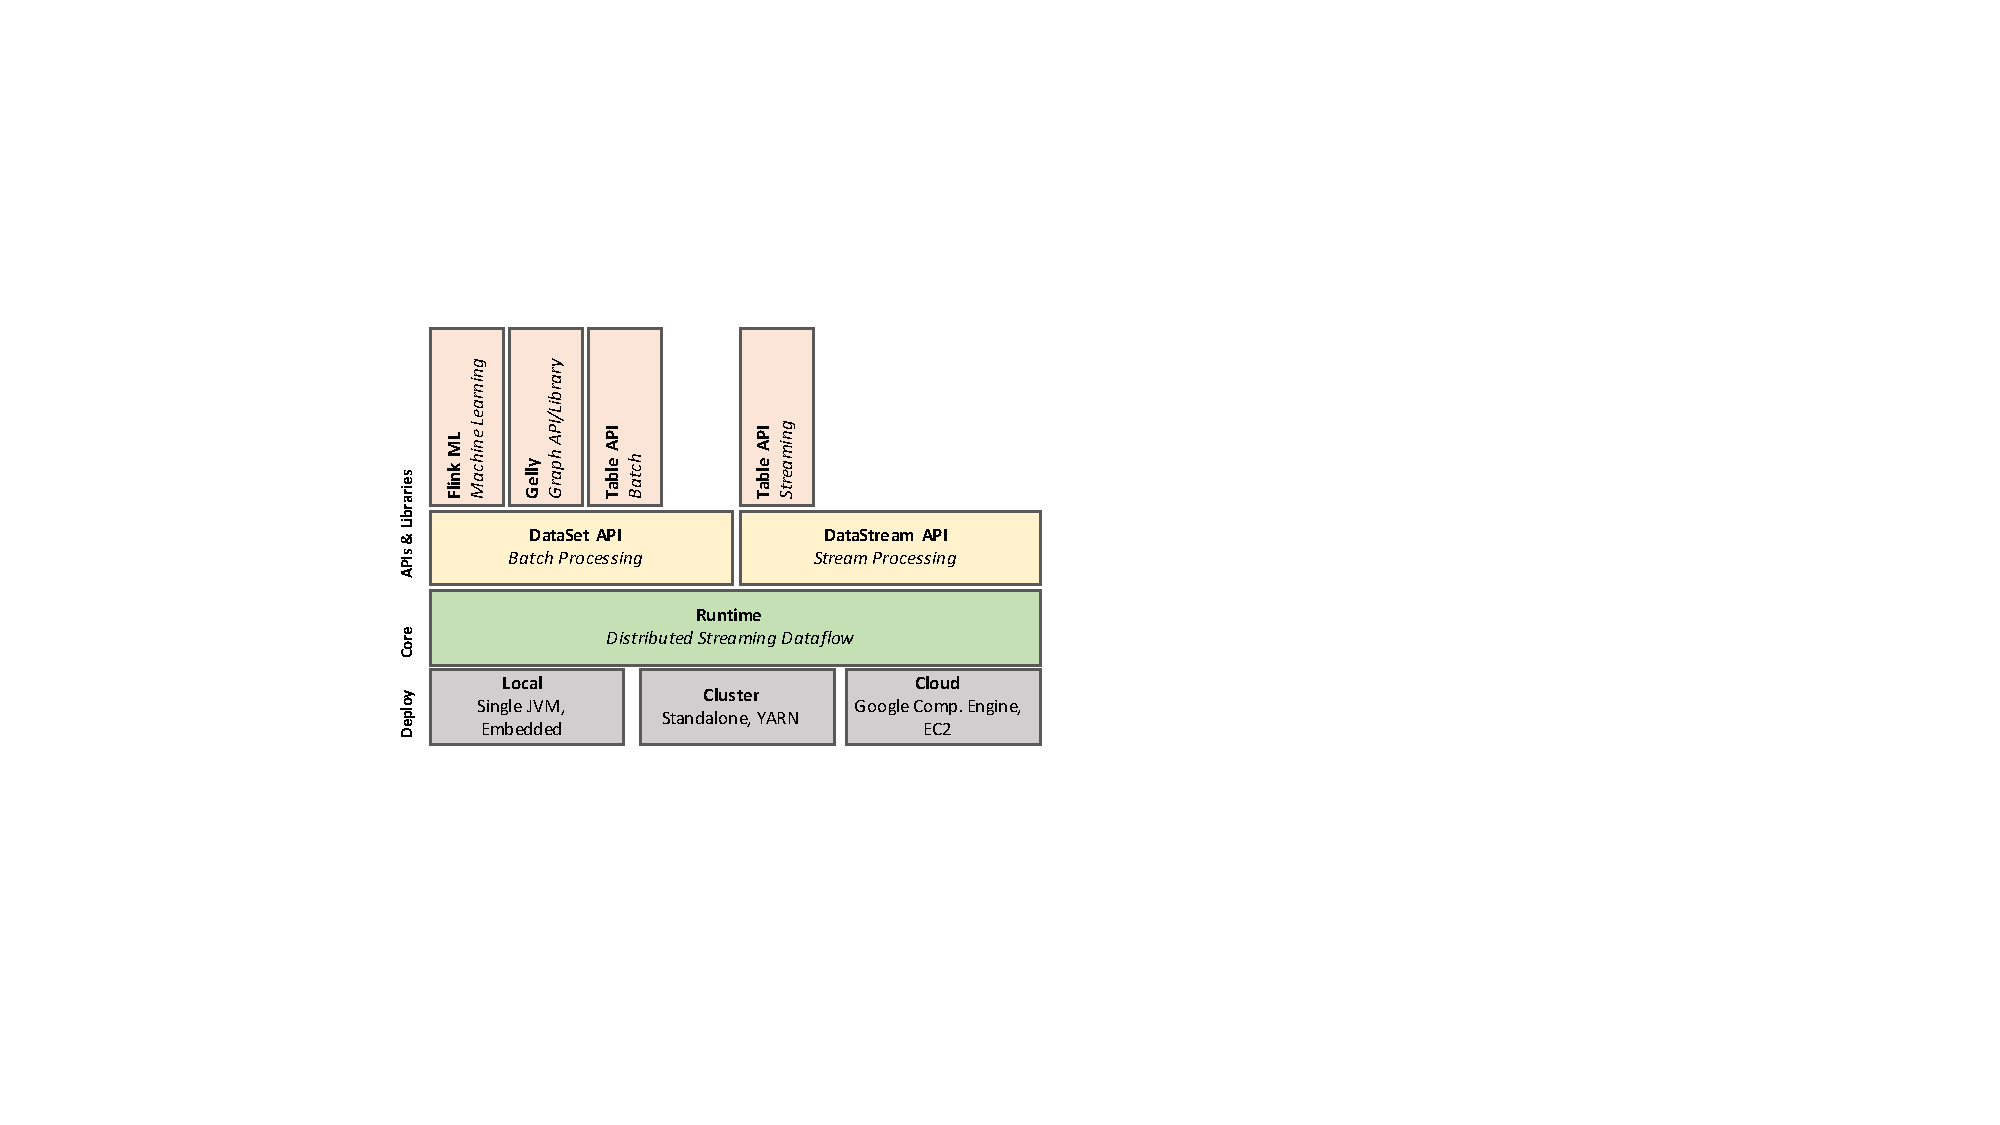
\includegraphics[width=.88\textwidth]{figs/stack}
			\caption{Flink's Software Stack.}
			\label{fig:stack}
          \end{figure}
      \end{minipage}
      % \hspace{0.05\linewidth}
      \begin{minipage}{0.48\linewidth}
          \begin{figure}[H]
				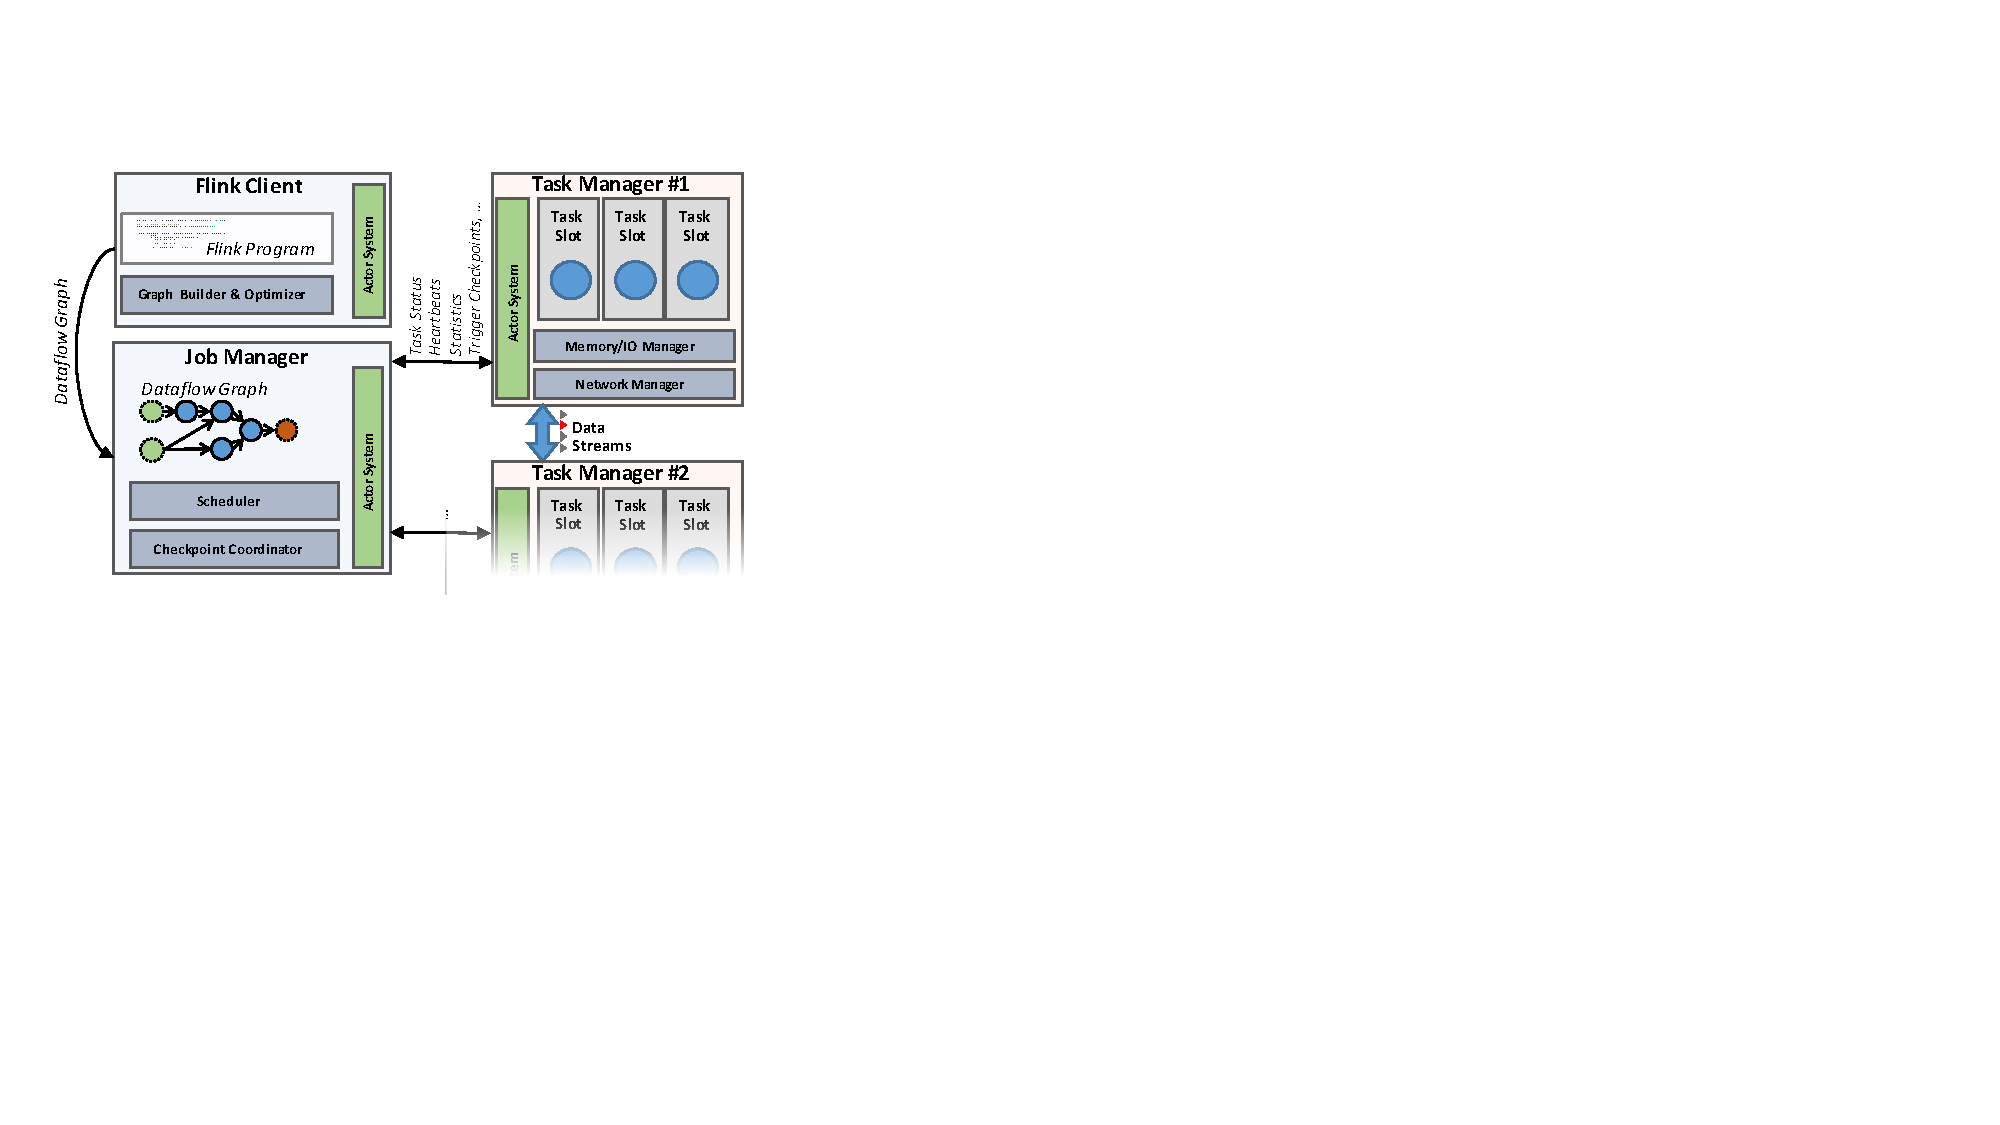
\includegraphics[width=.95\textwidth]{figs/architecture.pdf}
    			\caption{Flink's Process Model.}
    			\label{fig:process-model}
          \end{figure}
      \end{minipage}
  \end{minipage}
\end{figure}

